% Options for packages loaded elsewhere
\PassOptionsToPackage{unicode}{hyperref}
\PassOptionsToPackage{hyphens}{url}
%
\documentclass[
  8pt,
  ignorenonframetext,
]{beamer}
\usepackage{pgfpages}
\setbeamertemplate{caption}[numbered]
\setbeamertemplate{caption label separator}{: }
\setbeamercolor{caption name}{fg=normal text.fg}
\beamertemplatenavigationsymbolsempty
% Prevent slide breaks in the middle of a paragraph
\widowpenalties 1 10000
\raggedbottom
\setbeamertemplate{part page}{
  \centering
  \begin{beamercolorbox}[sep=16pt,center]{part title}
    \usebeamerfont{part title}\insertpart\par
  \end{beamercolorbox}
}
\setbeamertemplate{section page}{
  \centering
  \begin{beamercolorbox}[sep=12pt,center]{part title}
    \usebeamerfont{section title}\insertsection\par
  \end{beamercolorbox}
}
\setbeamertemplate{subsection page}{
  \centering
  \begin{beamercolorbox}[sep=8pt,center]{part title}
    \usebeamerfont{subsection title}\insertsubsection\par
  \end{beamercolorbox}
}
\AtBeginPart{
  \frame{\partpage}
}
\AtBeginSection{
  \ifbibliography
  \else
    \frame{\sectionpage}
  \fi
}
\AtBeginSubsection{
  \frame{\subsectionpage}
}
\usepackage{amsmath,amssymb}
\usepackage{lmodern}
\usepackage{iftex}
\ifPDFTeX
  \usepackage[T1]{fontenc}
  \usepackage[utf8]{inputenc}
  \usepackage{textcomp} % provide euro and other symbols
\else % if luatex or xetex
  \usepackage{unicode-math}
  \defaultfontfeatures{Scale=MatchLowercase}
  \defaultfontfeatures[\rmfamily]{Ligatures=TeX,Scale=1}
\fi
% Use upquote if available, for straight quotes in verbatim environments
\IfFileExists{upquote.sty}{\usepackage{upquote}}{}
\IfFileExists{microtype.sty}{% use microtype if available
  \usepackage[]{microtype}
  \UseMicrotypeSet[protrusion]{basicmath} % disable protrusion for tt fonts
}{}
\makeatletter
\@ifundefined{KOMAClassName}{% if non-KOMA class
  \IfFileExists{parskip.sty}{%
    \usepackage{parskip}
  }{% else
    \setlength{\parindent}{0pt}
    \setlength{\parskip}{6pt plus 2pt minus 1pt}}
}{% if KOMA class
  \KOMAoptions{parskip=half}}
\makeatother
\usepackage{xcolor}
\newif\ifbibliography
\usepackage{longtable,booktabs,array}
\usepackage{calc} % for calculating minipage widths
\usepackage{caption}
% Make caption package work with longtable
\makeatletter
\def\fnum@table{\tablename~\thetable}
\makeatother
\setlength{\emergencystretch}{3em} % prevent overfull lines
\providecommand{\tightlist}{%
  \setlength{\itemsep}{0pt}\setlength{\parskip}{0pt}}
\setcounter{secnumdepth}{-\maxdimen} % remove section numbering
\newlength{\cslhangindent}
\setlength{\cslhangindent}{1.5em}
\newlength{\csllabelwidth}
\setlength{\csllabelwidth}{3em}
\newlength{\cslentryspacingunit} % times entry-spacing
\setlength{\cslentryspacingunit}{\parskip}
\newenvironment{CSLReferences}[2] % #1 hanging-ident, #2 entry spacing
 {% don't indent paragraphs
  \setlength{\parindent}{0pt}
  % turn on hanging indent if param 1 is 1
  \ifodd #1
  \let\oldpar\par
  \def\par{\hangindent=\cslhangindent\oldpar}
  \fi
  % set entry spacing
  \setlength{\parskip}{#2\cslentryspacingunit}
 }%
 {}
\usepackage{calc}
\newcommand{\CSLBlock}[1]{#1\hfill\break}
\newcommand{\CSLLeftMargin}[1]{\parbox[t]{\csllabelwidth}{#1}}
\newcommand{\CSLRightInline}[1]{\parbox[t]{\linewidth - \csllabelwidth}{#1}\break}
\newcommand{\CSLIndent}[1]{\hspace{\cslhangindent}#1}
% type setting
% ------------------------------------------------------------------------------
\usepackage[german]{babel}     

% fonts
% ------------------------------------------------------------------------------
\usefonttheme{professionalfonts}

% slide title and horizontal line
% ------------------------------------------------------------------------------
\setbeamertemplate{frametitle}{%
    \vskip-30pt \color{black}\large%
    \begin{minipage}[b][23pt]{120mm}%
    \flushleft\insertframetitle%
    \end{minipage}%
}

\setbeamertemplate{headline}										
{
\vskip10pt\hfill\hspace{3.5mm} 										 
\vskip15pt\color{black}\rule{\textwidth}{0.4pt} 					 
}

% slide number
% ---------------------------------------------------------------
\setbeamertemplate{navigation symbols}{}
\setbeamertemplate{footline}
{
\vskip5pt
\vskip2pt
\makebox[123mm]{\hspace{7.5mm}
\hfill Multivariate Datenanalyse $\vert$ 
\copyright $ $ 2023 Dirk Ostwald CC BY-NC-SA 4.0 $\vert$ 
Folie \insertframenumber}
\vskip4pt
}

% block color scheme
% ------------------------------------------------------------------------------
% colors
\definecolor{white}{RGB}{255,255,255}
\definecolor{grey}{RGB}{235,235,235}
\definecolor{lightgrey}{RGB}{245,245,245}
\definecolor{LightBlue}{RGB}{220,220,255}
\definecolor{darkblue}{RGB}{51, 51, 153}

% definitions and theorems
\setbeamercolor{block title}{fg = black, bg = grey}
\setbeamercolor{block body}{fg = black, bg = lightgrey}

% general line spacing 
% ------------------------------------------------------------------------------
\linespread{1.3}

% local line spacing
% ------------------------------------------------------------------------------
\usepackage{setspace}

% colors
% -----------------------------------------------------------------------------
\usepackage{color}

% justified text
% ------------------------------------------------------------------------------
\usepackage{ragged2e}
\usepackage{etoolbox}
\apptocmd{\frame}{}{\justifying}{}

% bullet point lists
% -----------------------------------------------------------------------------
\setbeamertemplate{itemize item}[circle]
\setbeamertemplate{itemize subitem}[circle]
\setbeamertemplate{itemize subsubitem}[circle]
\setbeamercolor{itemize item}{fg = black}
\setbeamercolor{itemize subitem}{fg = black}
\setbeamercolor{itemize subsubitem}{fg = black}
\setbeamercolor{enumerate item}{fg = black}
\setbeamercolor{enumerate subitem}{fg = black}
\setbeamercolor{enumerate subsubitem}{fg = black}
\setbeamerfont{itemize/enumerate body}{}
\setbeamerfont{itemize/enumerate subbody}{size = \normalsize}
\setbeamerfont{itemize/enumerate subsubbody}{size = \normalsize}

% color links
% ------------------------------------------------------------------------------
\usepackage{hyperref}
\definecolor{urls}{RGB}{204,0,0}
\hypersetup{colorlinks, citecolor = darkblue, urlcolor = urls}


% additional math commands
% ------------------------------------------------------------------------------
\usepackage{bm}                                         % bold math symbols
\newcommand{\niton}{\not\owns}

% text highlighting
% ------------------------------------------------------------------------------
\usepackage{soul}
\makeatletter
\let\HL\hl
\renewcommand\hl{%
  \let\set@color\beamerorig@set@color
  \let\reset@color\beamerorig@reset@color
  \HL}
\makeatother

% equation highlighting
% -----------------------------------------------------------------------------
\newcommand{\highlight}[2][yellow]{\mathchoice%
  {\colorbox{#1}{$\displaystyle#2$}}%
  {\colorbox{#1}{$\textstyle#2$}}%
  {\colorbox{#1}{$\scriptstyle#2$}}%
  {\colorbox{#1}{$\scriptscriptstyle#2$}}}%

% additional mathematical operators
% ------------------------------------------------------------------------------
\DeclareMathOperator*{\argmax}{arg\,max}
\DeclareMathOperator*{\argmin}{arg\,min}

\ifLuaTeX
  \usepackage{selnolig}  % disable illegal ligatures
\fi
\IfFileExists{bookmark.sty}{\usepackage{bookmark}}{\usepackage{hyperref}}
\IfFileExists{xurl.sty}{\usepackage{xurl}}{} % add URL line breaks if available
\urlstyle{same} % disable monospaced font for URLs
\hypersetup{
  hidelinks,
  pdfcreator={LaTeX via pandoc}}

\author{}
\date{\vspace{-2.5em}}

\begin{document}

\begin{frame}[plain]{}
\protect\hypertarget{section}{}
\center

\begin{center}
\includegraphics[width=0.2\linewidth]{1_Abbildungen/mvda_1_otto} \end{center}

\vspace{2mm}

\Huge

Multivariate Datenanalyse \vspace{6mm}

\Large

MSc Psychologie WiSe 2022/23

\vspace{6mm}
\large

Prof.~Dr.~Dirk Ostwald
\end{frame}

\begin{frame}[plain]{}
\protect\hypertarget{section-1}{}
\vfill
\center
\huge

\textcolor{red}{Aufnahme läuft!} \vfill
\end{frame}

\begin{frame}[plain]{}
\protect\hypertarget{section-2}{}
\vfill
\center
\huge

\textcolor{black}{(1) Einführung} \vfill
\end{frame}

\begin{frame}[plain]{}
\protect\hypertarget{section-3}{}
\vfill
\begin{large}
Prof. Dr. Dirk Ostwald (dirk.ostwald@ovgu.de)
\end{large}
\vspace{.7cm}

\begin{minipage}{.3\linewidth}
\begin{center}
\includegraphics[scale=.6]{1_Abbildungen/mvda_1_dirk.pdf}
\end{center}
\end{minipage}
\begin{minipage}{.7\linewidth}
\begin{small}
\renewcommand{\arraystretch}{1.3}
\begin{tabular}{ll}
Seit 2021   & W2 Professur Methodenlehre I              \\
2014 - 2020 & W1 Professur Freie Universität Berlin     \\
2010 - 2014 & Postdoc BCCN \& MPIB Berlin               \\
2007 - 2010 & PhD Psychologie Birmingham                \\
2004 - 2006 & MSc Neurowissenschaften Tübingen          \\
2005 - 2012 & BSc Mathematik Hagen                      \\
2000 - 2003 & BSc Medizin Hamburg                       \\
\end{tabular}
\end{small}
\end{minipage}
\vspace{.7cm}

\begin{large}
\begin{tabular}{ll}
Forschung   & Komputationale Kognitive Neurowissenschaften  \\
Lehre       & Datenwissenschaft
\end{tabular}
\end{large}
\vfill
\end{frame}

\begin{frame}{}
\protect\hypertarget{section-4}{}
\href{https://www.ipsy.ovgu.de/methodenlehre_I-path-980,1404.html}{\textcolor{darkblue}{Homepage}}

\begin{center}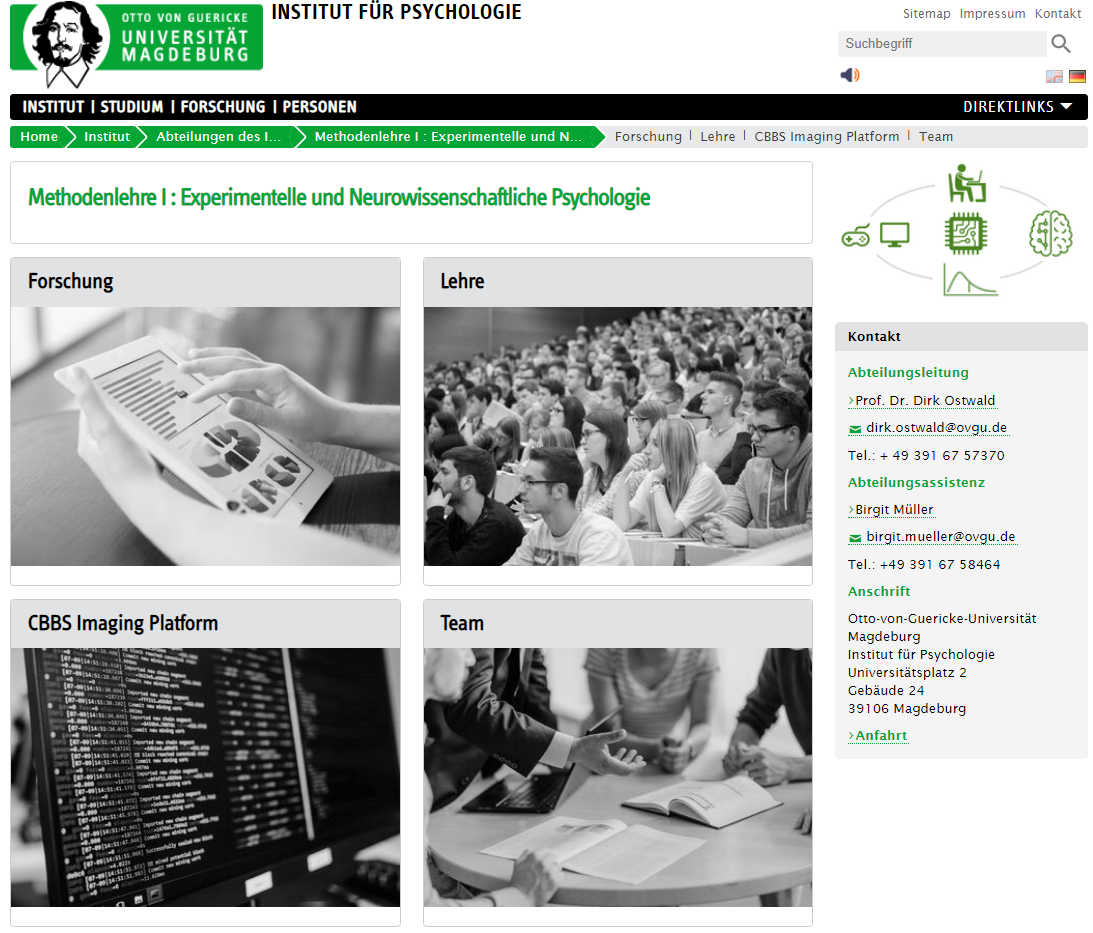
\includegraphics[width=0.7\linewidth]{1_Abbildungen/mvda_1_homepage} \end{center}
\end{frame}

\begin{frame}{}
\protect\hypertarget{section-5}{}
\setstretch{3}
\vfill
\Large

Motivation

Datenwissenschaft

Formalia \vfill
\end{frame}

\begin{frame}{}
\protect\hypertarget{section-6}{}
\setstretch{3}
\vfill
\Large

\textbf{Motivation}

Datenwissenschaft

Formalia \vfill
\end{frame}

\begin{frame}{Motivation}
\protect\hypertarget{motivation}{}
\setstretch{1.5}
\large

\textcolor{darkblue}{Multivariate Verfahren}

\normalsize

\begin{itemize}
\item
  Einblick in die moderne multivariate Datenanalyse
\item
  Methoden der Statistik und des Maschinellen Lernens
\end{itemize}

\small

\begin{longtable}[]{@{}
  >{\raggedright\arraybackslash}p{(\columnwidth - 4\tabcolsep) * \real{0.3108}}
  >{\raggedright\arraybackslash}p{(\columnwidth - 4\tabcolsep) * \real{0.4324}}
  >{\raggedright\arraybackslash}p{(\columnwidth - 4\tabcolsep) * \real{0.2568}}@{}}
\toprule()
\begin{minipage}[b]{\linewidth}\raggedright
\end{minipage} & \begin{minipage}[b]{\linewidth}\raggedright
Unabhängige Variable
\end{minipage} & \begin{minipage}[b]{\linewidth}\raggedright
Abhängige Variable
\end{minipage} \\
\midrule()
\endhead
Univariate Verfahren & Eindimensional, mehrdimensional &
Eindimensional \\
Multivariate Verfahren & Eindimensional, mehrdimensional &
Mehrdimensional \\
\bottomrule()
\end{longtable}

\normalsize

\begin{itemize}
\item
  Grundlagen (Vektoren, Matrizen, Eigenanalyse, Multivariate
  Normalverteilung)
\item
  Verfahren der Datenreduktion (Hauptkomponentenanalyse, Faktoranalyse)
\item
  Verfahren der frequentistischen Inferenz (ANOVA, Regression,
  Korrelation)
\item
  Verfahren der Klassifikation (Logistische Regression, SVMs, Neuronale
  Netze)
\end{itemize}
\end{frame}

\begin{frame}{Motivation}
\protect\hypertarget{motivation-1}{}
\textcolor{darkblue}{Neurobiologische Verarbeitung von Sinnesreizen}

\normalsize

Wie werden visuelle Stimuli im Gerhin verarbeitet?

Wie entscheiden Menschen, ob sie ein Haus oder ein Gesicht wahrnehmen?

\begin{center}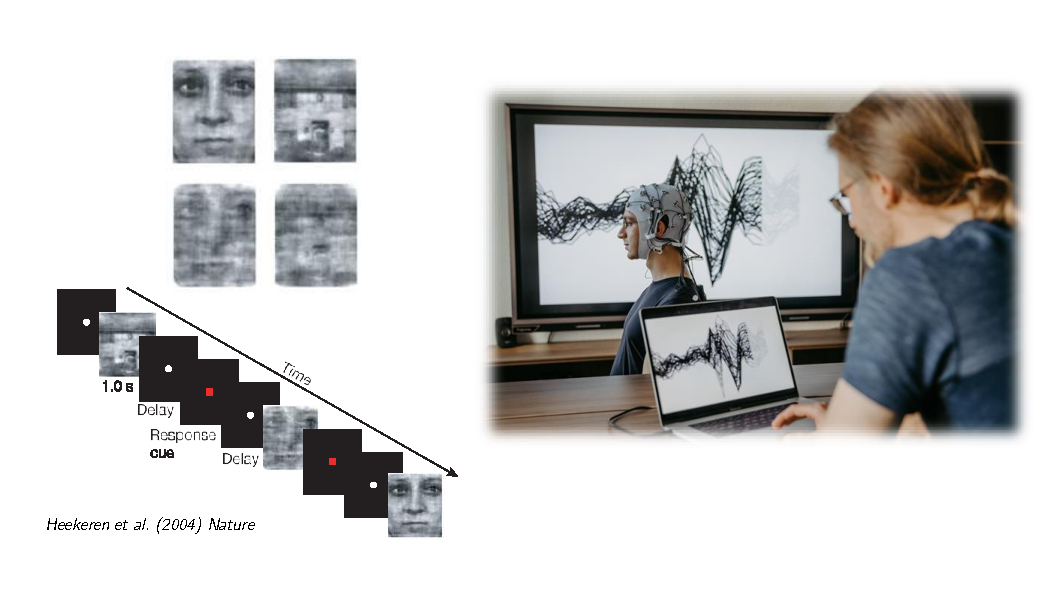
\includegraphics[width=0.8\linewidth]{1_Abbildungen/mvda_1_neurosensorik} \end{center}

\(\rightarrow\) Allgemeine Psychologie, Biologische Psychologie,
Kognitive Neurowissenschaften
\end{frame}

\begin{frame}{Motivation}
\protect\hypertarget{motivation-2}{}
\textcolor{darkblue}{Neurobiologische Verarbeitung von Sinnesreizen - Verhaltensdaten}

\footnotesize

\begin{longtable}[]{@{}ccccc@{}}
\toprule()
Trial & Stimulus & Kohärenz & Antwort & Reaktionszeit (ms) \\
\midrule()
\endhead
1 & Gesicht & 20 & Gesicht & 854 \\
2 & Gesicht & 20 & Haus & 843 \\
3 & Haus & 60 & Gesicht & 369 \\
4 & Gesicht & 60 & Haus & 564 \\
5 & Gesicht & 20 & Haus & 449 \\
6 & Haus & 40 & Gesicht & 565 \\
7 & Gesicht & 40 & Gesicht & 715 \\
8 & Gesicht & 60 & Haus & 416 \\
9 & Gesicht & 60 & Haus & 828 \\
10 & Haus & 40 & Haus & 479 \\
11 & Haus & 60 & Gesicht & 483 \\
12 & Gesicht & 20 & Gesicht & 321 \\
\bottomrule()
\end{longtable}

\normalsize
\center

Unabhängige Variable = (Stimulus, Kohärenz)

Abhängige Variable = (Antwort, Reaktionszeit)
\end{frame}

\begin{frame}{Motivation}
\protect\hypertarget{motivation-3}{}
\textcolor{darkblue}{Neurobiologische Verarbeitung von Sinnesreizen - Neurophysiologiedaten}

\footnotesize

\begin{longtable}[]{@{}
  >{\centering\arraybackslash}p{(\columnwidth - 14\tabcolsep) * \real{0.0571}}
  >{\centering\arraybackslash}p{(\columnwidth - 14\tabcolsep) * \real{0.1429}}
  >{\centering\arraybackslash}p{(\columnwidth - 14\tabcolsep) * \real{0.1286}}
  >{\centering\arraybackslash}p{(\columnwidth - 14\tabcolsep) * \real{0.1286}}
  >{\centering\arraybackslash}p{(\columnwidth - 14\tabcolsep) * \real{0.1286}}
  >{\centering\arraybackslash}p{(\columnwidth - 14\tabcolsep) * \real{0.1286}}
  >{\centering\arraybackslash}p{(\columnwidth - 14\tabcolsep) * \real{0.1429}}
  >{\centering\arraybackslash}p{(\columnwidth - 14\tabcolsep) * \real{0.1429}}@{}}
\toprule()
\begin{minipage}[b]{\linewidth}\centering
ms
\end{minipage} & \begin{minipage}[b]{\linewidth}\centering
Stimulus
\end{minipage} & \begin{minipage}[b]{\linewidth}\centering
E1 (O1)
\end{minipage} & \begin{minipage}[b]{\linewidth}\centering
E2 (O2)
\end{minipage} & \begin{minipage}[b]{\linewidth}\centering
E3 (Cz)
\end{minipage} & \begin{minipage}[b]{\linewidth}\centering
E4 (Pz)
\end{minipage} & \begin{minipage}[b]{\linewidth}\centering
E5 (AF1)
\end{minipage} & \begin{minipage}[b]{\linewidth}\centering
E6 (AF2)
\end{minipage} \\
\midrule()
\endhead
0 & Gesicht & -0.827 & -0.063 & -2.26 & -1.50 & -0.537 & 1.34 \\
2 & Gesicht & 15.317 & 16.571 & 19.52 & 17.09 & 17.946 & 16.54 \\
4 & Gesicht & 19.121 & 18.636 & 17.82 & 19.54 & 15.569 & 17.79 \\
6 & Gesicht & 2.999 & 5.590 & 3.02 & 3.09 & 2.656 & 2.02 \\
8 & Gesicht & -14.892 & -15.081 & -14.07 & -13.80 & -14.709 & -16.20 \\
10 & Gesicht & -17.555 & -18.604 & -19.84 & -18.66 & -19.557 & -19.97 \\
12 & Gesicht & -5.477 & -5.482 & -4.46 & -5.01 & -5.153 & -7.33 \\
14 & Gesicht & 13.005 & 11.218 & 12.90 & 13.00 & 14.211 & 12.46 \\
16 & Gesicht & 17.877 & 20.651 & 18.61 & 19.96 & 20.834 & 19.23 \\
18 & Gesicht & 7.963 & 8.011 & 7.26 & 8.18 & 8.194 & 7.69 \\
20 & Gesicht & -11.194 & -11.076 & -9.82 & -8.93 & -10.404 & -10.67 \\
22 & Gesicht & -18.932 & -19.981 & -19.87 & -18.70 & -18.327 & -19.02 \\
24 & Gesicht & -10.662 & -10.713 & -10.23 & -10.01 & -11.076 & -10.92 \\
\bottomrule()
\end{longtable}

\normalsize
\center

Unabhängige Variable = (Stimulus)

Abhängige Variable = (E1,E2,E3,E4,E5,E6)
\end{frame}

\begin{frame}{Motivation}
\protect\hypertarget{motivation-4}{}
\textcolor{darkblue}{Evidenzbasierte Evaluation von Psychotherapieformen bei Depression}

\normalsize

Welche Therapieform ist bei Depression wirksamer?

\begin{center}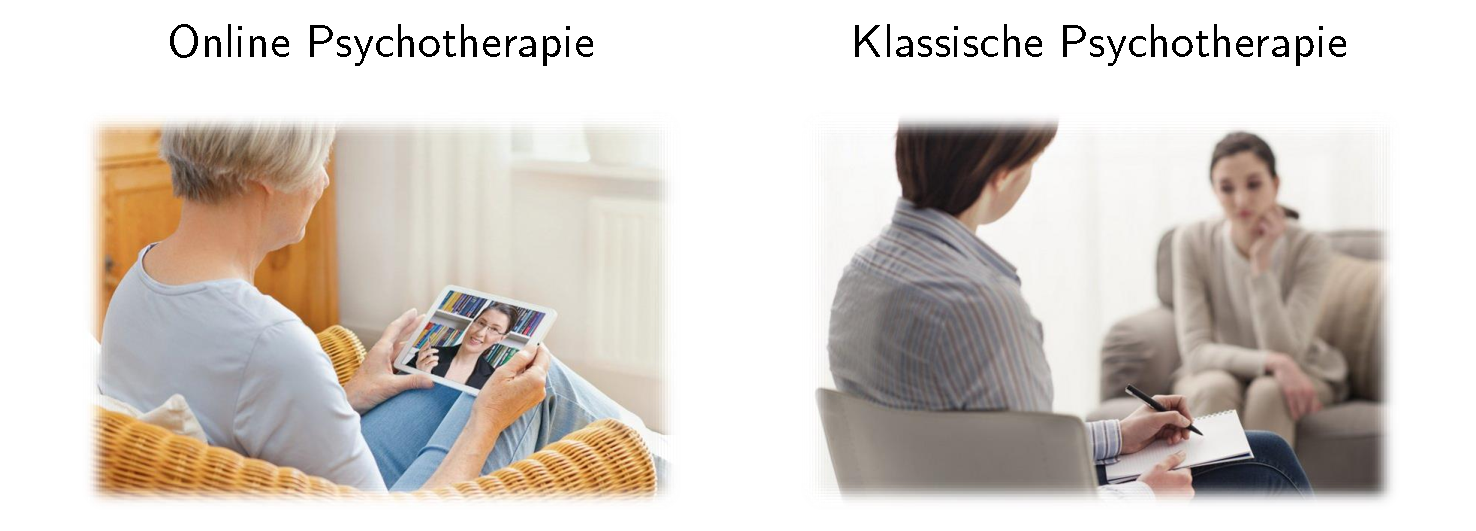
\includegraphics[width=1.1\linewidth]{1_Abbildungen/mvda_1_klinische_forschung} \end{center}

\(\rightarrow\) Klinische Psychologie, Klinische Diagnostik
\end{frame}

\begin{frame}{Motivation}
\protect\hypertarget{motivation-5}{}
\textcolor{darkblue}{Evidenzbasierte Evaluation von Psychotherapieformen bei Depression}

\footnotesize

\begin{longtable}[]{@{}
  >{\centering\arraybackslash}p{(\columnwidth - 10\tabcolsep) * \real{0.1379}}
  >{\centering\arraybackslash}p{(\columnwidth - 10\tabcolsep) * \real{0.1264}}
  >{\centering\arraybackslash}p{(\columnwidth - 10\tabcolsep) * \real{0.1149}}
  >{\centering\arraybackslash}p{(\columnwidth - 10\tabcolsep) * \real{0.1149}}
  >{\centering\arraybackslash}p{(\columnwidth - 10\tabcolsep) * \real{0.2529}}
  >{\centering\arraybackslash}p{(\columnwidth - 10\tabcolsep) * \real{0.2529}}@{}}
\toprule()
\begin{minipage}[b]{\linewidth}\centering
Patient ID
\end{minipage} & \begin{minipage}[b]{\linewidth}\centering
Bedingung
\end{minipage} & \begin{minipage}[b]{\linewidth}\centering
Prae BDI
\end{minipage} & \begin{minipage}[b]{\linewidth}\centering
Post BDI
\end{minipage} & \begin{minipage}[b]{\linewidth}\centering
Prae Glukokortikoide
\end{minipage} & \begin{minipage}[b]{\linewidth}\centering
Post Glukokortikoide
\end{minipage} \\
\midrule()
\endhead
1 & Online & 25 & 10 & 192 & 197 \\
2 & Online & 21 & 30 & 372 & 200 \\
3 & Online & 42 & 11 & 209 & 233 \\
4 & Online & 26 & 18 & 212 & 150 \\
5 & Online & 17 & 20 & 468 & 212 \\
6 & Online & 30 & 10 & 339 & 267 \\
7 & Online & 22 & 25 & 183 & 299 \\
8 & Online & 26 & 24 & 399 & 241 \\
9 & Online & 16 & 20 & 191 & 166 \\
10 & Klassisch & 21 & 29 & 455 & 117 \\
11 & Online & 32 & 10 & 168 & 242 \\
12 & Online & 40 & 19 & 233 & 191 \\
\bottomrule()
\end{longtable}

\center
\normalsize

Unabhängige Variable = (Bedingung)

Abhängige Variable = (\(\Delta\)BDI, \(\Delta\)Glukokortikoide)
\end{frame}

\begin{frame}{Motivation}
\protect\hypertarget{motivation-6}{}
\textcolor{darkblue}{Approbationsordnung für Psychotherapeutinnen und Psychotherapeuten (2020)}

\small

Inhalte, die im Masterstudiengang im Rahmen der hochschulischen Lehre zu
vermitteln und bei dem Antrag auf Zulassung zur psychotherapeutischen
Prüfung nachzuweisen sind \vspace{2mm}

\footnotesize

\noindent \textbf{2. vertiefte Forschungsmethodik}

Die studierenden Personen

\begin{enumerate}
[a)]
\item
  wenden komplexe und multivariate Erhebungs- und Auswertungsmethoden
  zur Evaluierung und Qualitätssicherung von Interventionen an,
\item
  nutzen und beurteilen einschlägige Forschungsstudien und deren
  Ergebnisse für die Psychotherapie
\item
  planen selbstständig Studien zur Neu- oder Weiterentwicklung der
  Psychotherapieforschung oder der Forschung in angrenzenden Bereichen,
  führen solche Studien durch, werten sie aus und fassen sie zusammen,
  (\ldots)
\end{enumerate}

\textcolor{blue}{$\quad\Rightarrow$ Masterarbeit}

Zur Vermittlung der Inhalte der vertieften Forschnungsmethodik sind bei
der Planung der hochschulischen Lehre (\ldots) die folgenden
Wissensbereiche abzudecken (\ldots)

\begin{enumerate}
[a)]
\tightlist
\item
  multivariate Verfahren und Messtheorie
\end{enumerate}
\end{frame}

\begin{frame}{}
\protect\hypertarget{section-7}{}
\setstretch{3}
\vfill
\Large

Motivation

\textbf{Datenwissenschaft}

Formalia \vfill
\end{frame}

\begin{frame}{Datenwissenschaft}
\protect\hypertarget{datenwissenschaft}{}
\vfill

\center
\huge

\textcolor{darkblue}{Datenwissenschaft} \vspace{5mm}

\Large

Die Kunst, aus Daten Sinn zu generieren
\end{frame}

\begin{frame}{Datenwissenschaft}
\protect\hypertarget{datenwissenschaft-1}{}
\vspace{2mm}

\begin{center}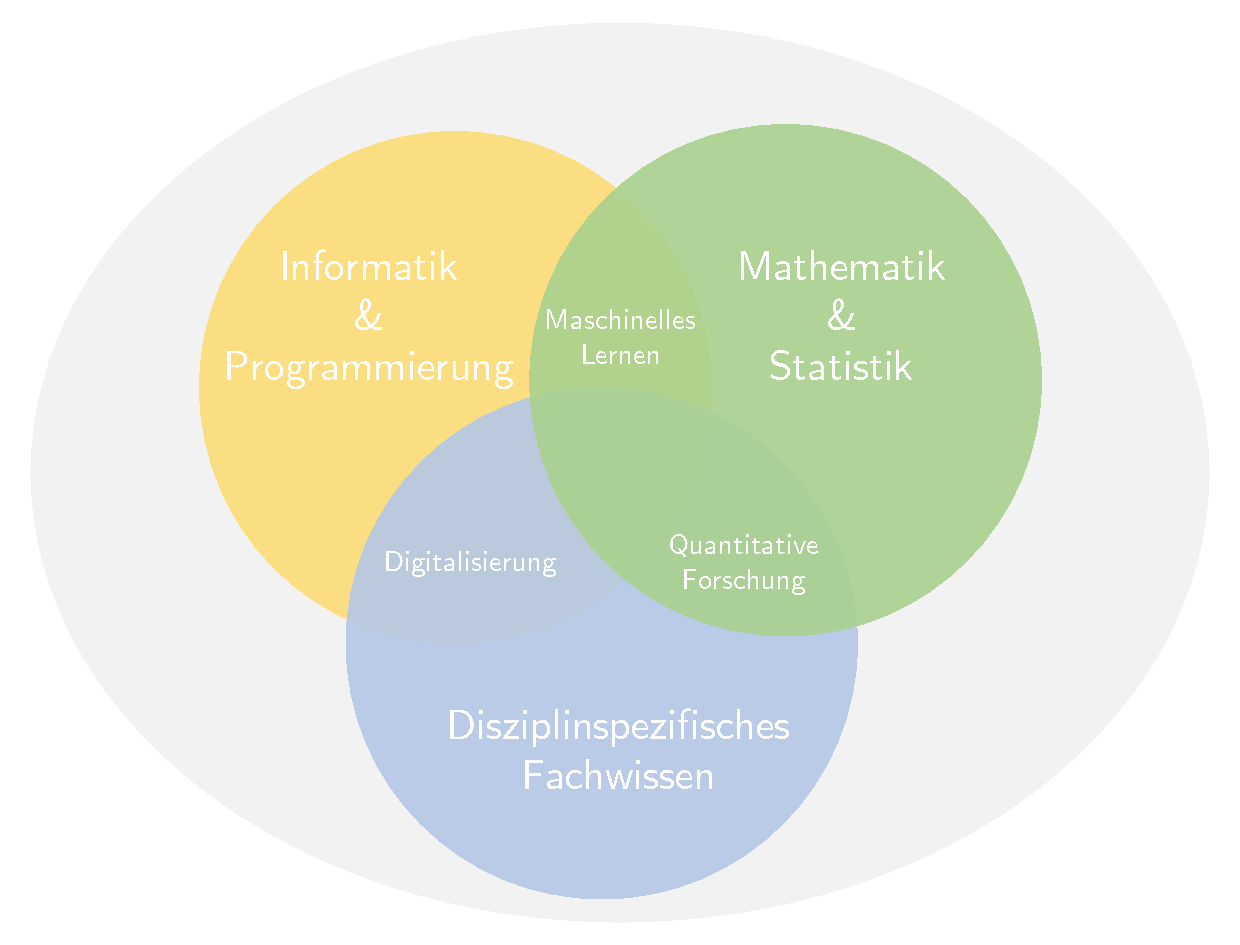
\includegraphics[width=0.9\linewidth]{1_Abbildungen/mvda_1_datenwissenschaft_komponenten} \end{center}
\vfill
\end{frame}

\begin{frame}{Datenwissenschaft}
\protect\hypertarget{datenwissenschaft-2}{}
\Large

Datenwissenschaft ist Datenreduktion

\center
\vspace{.4cm}

\begin{center}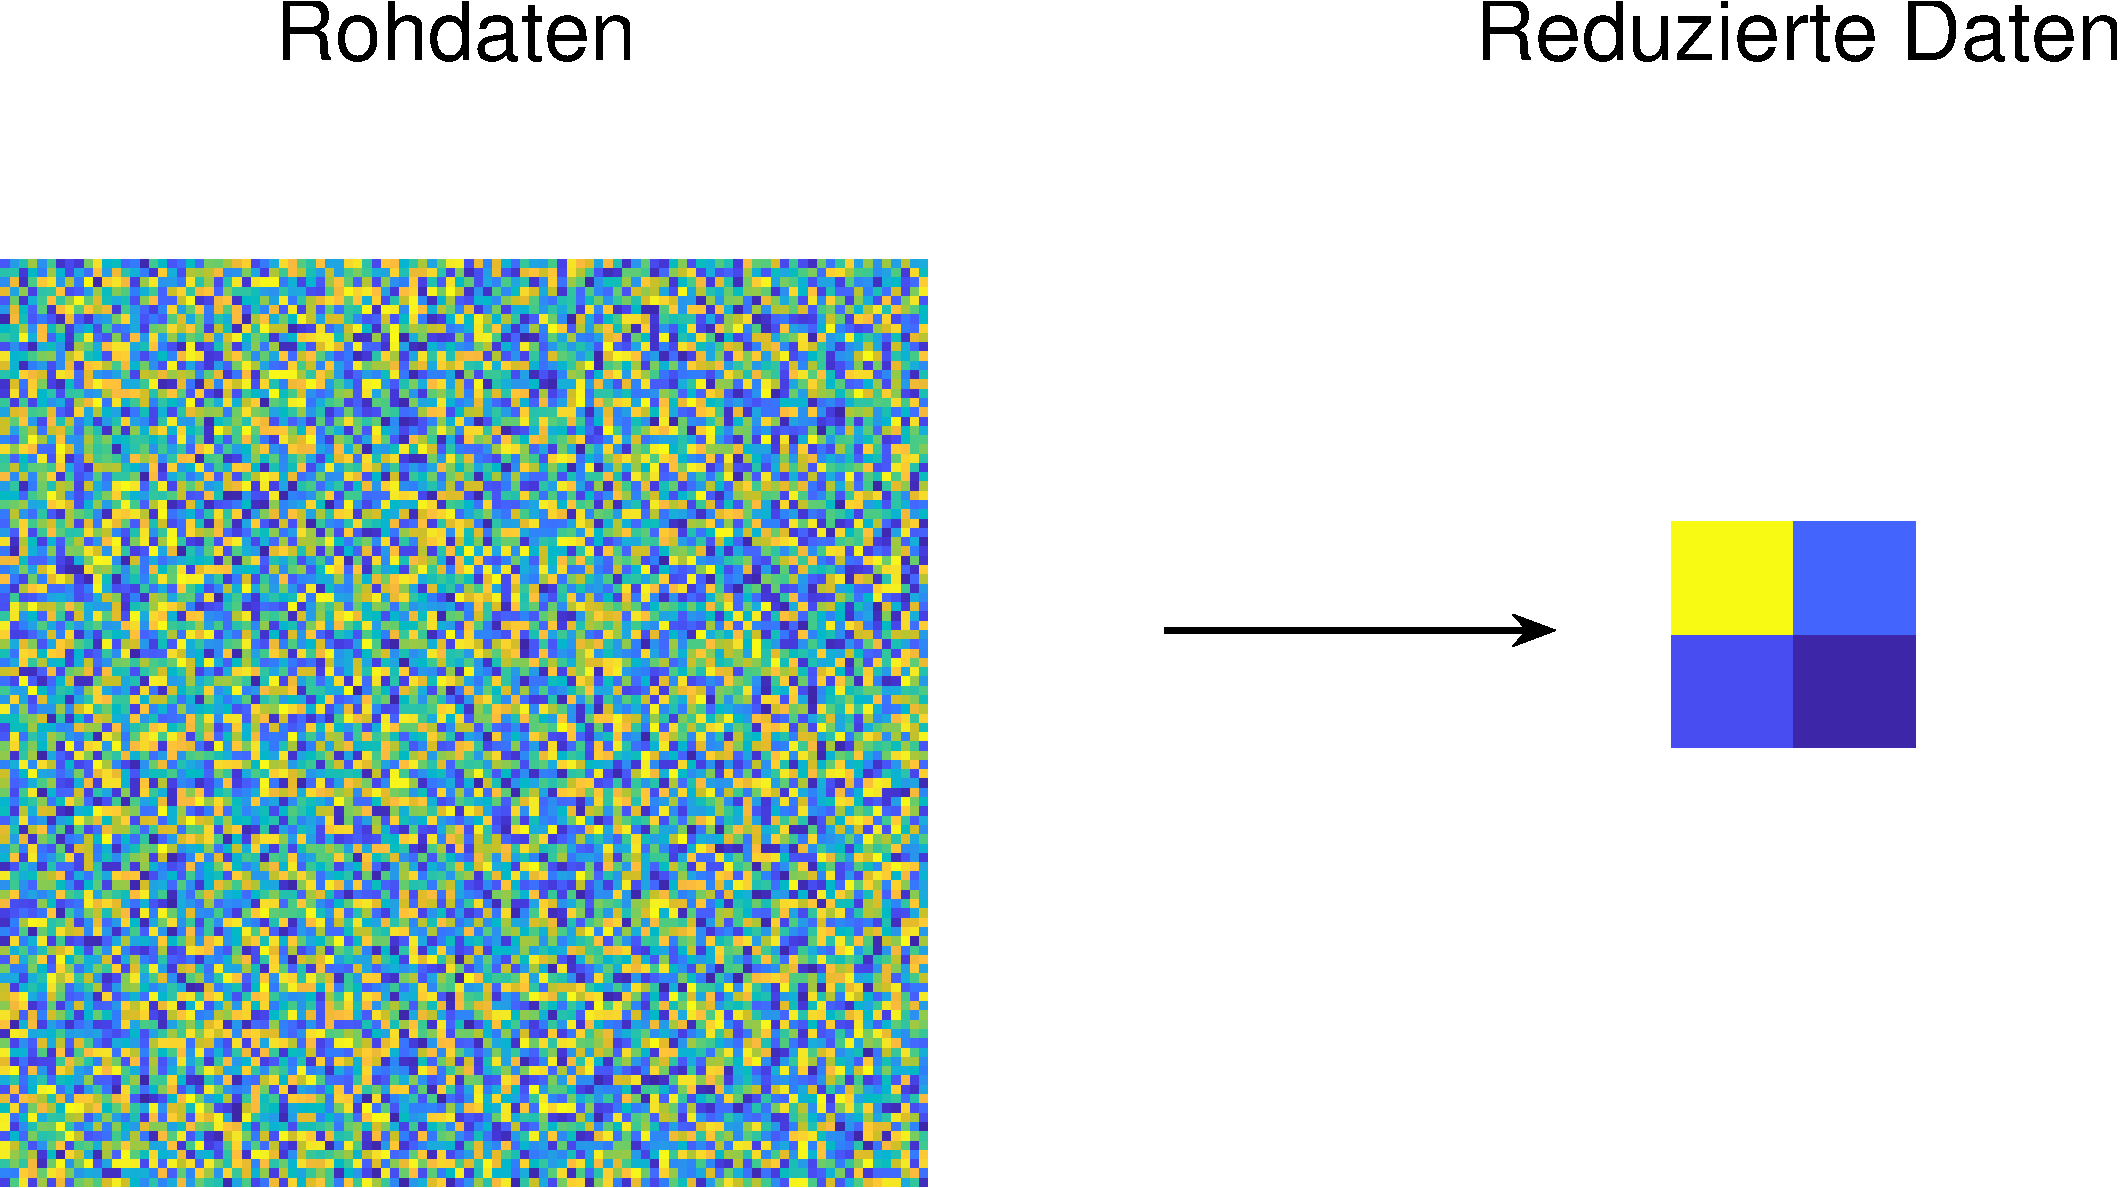
\includegraphics[width=0.8\linewidth]{1_Abbildungen/mvda_1_datenreduktion} \end{center}
\end{frame}

\begin{frame}{Datenwissenschaft}
\protect\hypertarget{datenwissenschaft-3}{}
\Large

Datenwissenschaft ist Naturwissenschaft \vspace{3mm}

\begin{center}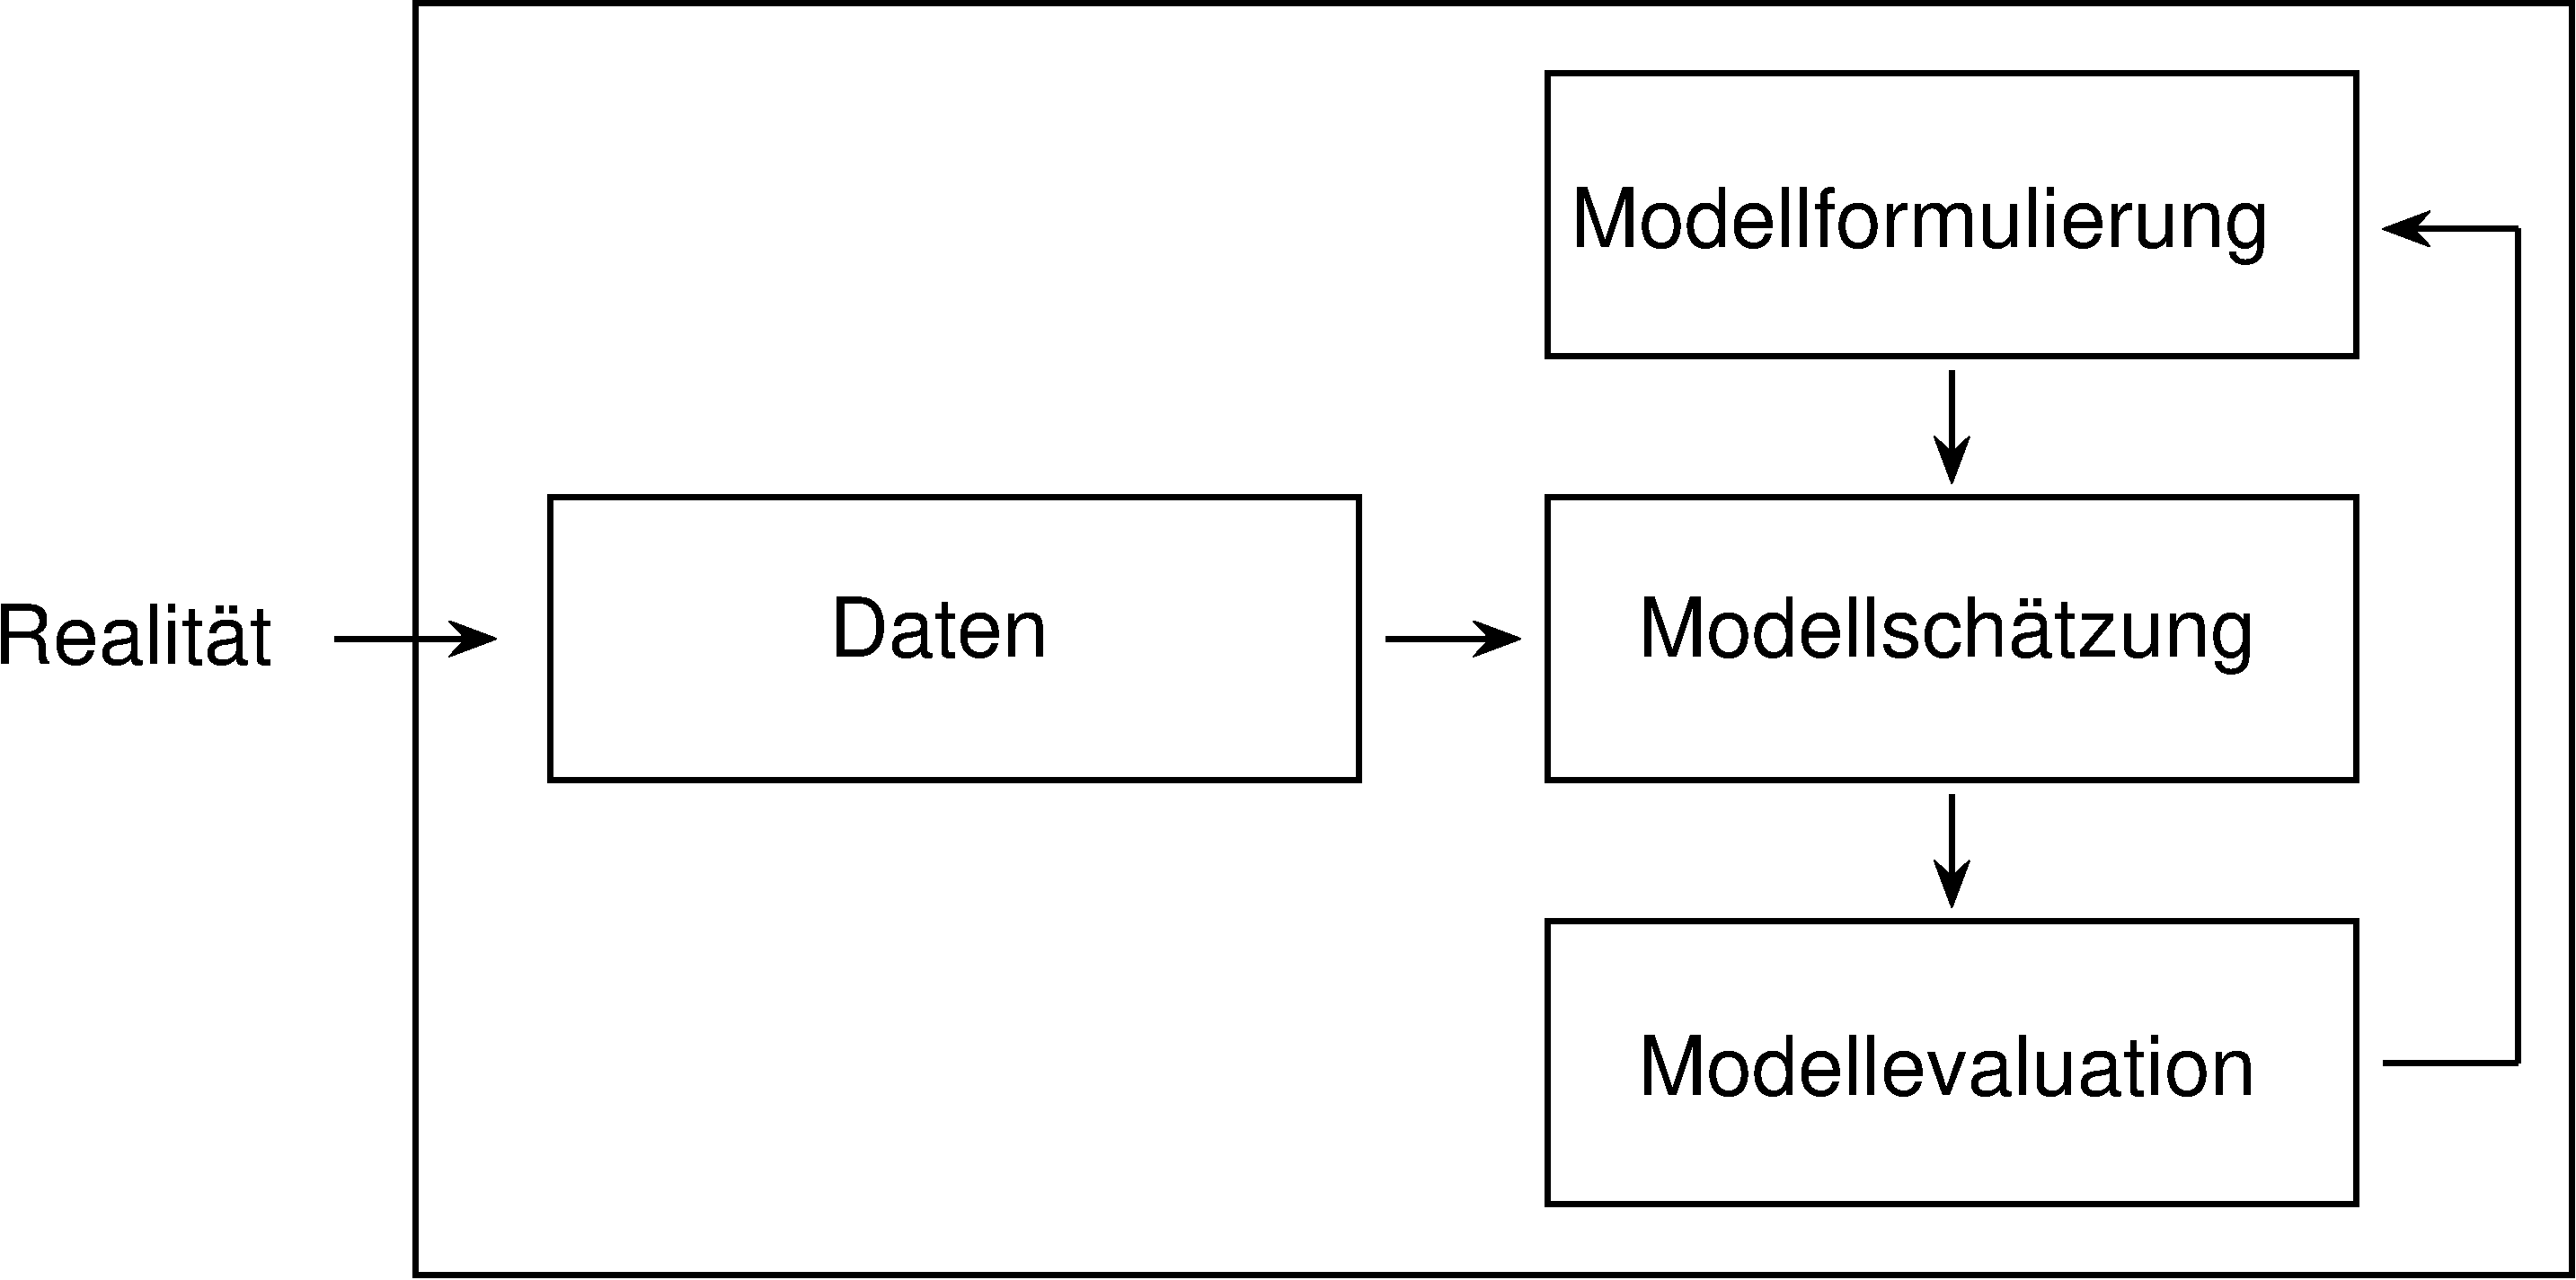
\includegraphics[width=1\linewidth]{1_Abbildungen/mvda_1_wissenschaft} \end{center}
\end{frame}

\begin{frame}{Datenwissenschaft}
\protect\hypertarget{datenwissenschaft-4}{}
\Large

Datenwissenchaft ist Dateninterpretation \center \vspace{.5cm}

\begin{center}
\includegraphics[width=0.8\linewidth]{1_Abbildungen/mvda_1_datenwissenschaftslinse} \end{center}
\end{frame}

\begin{frame}{Datenwissenschaft}
\protect\hypertarget{datenwissenschaft-5}{}
\Large

Terminologie der Datenwissenschaft \vspace{.5cm}

\center

Statistik = Maschinelles Lernen = Künstliche Intelligenz \vspace{.5cm}

\small
\renewcommand{\arraystretch}{1.5}
\begin{tabular}{l|l|l}

Statistik                           & Maschinelles Lernen           & Künstliche Intelligenz        \\\hline
Probabilistische Modelle    & Deterministische Modelle  & Agenten-basierte Modelle  \\
Theoretische Analyse          & Klassifikation                & Reinforcement learning      \\
Optimalitätstheorie           & Bayesianische Modelle         & Symbolik                              \\
Asymptotische Theorie         & Anwendung                           & Anwendung                           \\
Wissenschaftsphilosophie    & Benchmarking                    & Hype                                    \\
\end{tabular}
\end{frame}

\begin{frame}{Datenwissenschaft}
\protect\hypertarget{datenwissenschaft-6}{}
\vfill

\center
\huge

\textcolor{darkblue}{Datenwissenschaft in der Psychologie} \vspace{5mm}

\Large

Die Kunst, aus Verhaltens- und Neurophysiologiedaten

psychologischen Sinn zu generieren
\end{frame}

\begin{frame}{}
\protect\hypertarget{section-8}{}
\setstretch{3}
\vfill
\Large

Motivation

Datenwissenschaft

\textbf{Formalia} \vfill
\end{frame}

\begin{frame}{Formalia}
\protect\hypertarget{formalia}{}
\textcolor{darkblue}{Modul A1/A3 Forschungsmethoden: Multivariate Verfahren}
\setstretch{2.2}

\begin{itemize}
\tightlist
\item
  Live Freitags 9-11 Uhr in G40B-326 und 11-13 Uhr G40B-238
\item
  Kursmaterialien (Folien, Videos) auf der
  \href{https://bit.ly/3Eye26S}{\textcolor{darkblue}{Kurswebseite}}
\item
  Code auf
  \href{https://github.com/dirk-ostwald/multivariate-datenanalyse-23}{\textcolor{darkblue}{Github}}
\item
  Ankündigen über
  \href{https://elearning.ovgu.de/course/view.php?id=13782}{\textcolor{darkblue}{Moodle}}
\item
  \href{https://bit.ly/3DAw0Dg}{\textcolor{darkblue}{Link zur vorherigen Iteration des Kurses}}
\item
  \href{https://bit.ly/3SNh3nR}{\textcolor{darkblue}{Link zum Mathematik Grundlagenkurs des BSc Psychologie}}
\item
  \href{https://bit.ly/3MvFcwi}{\textcolor{darkblue}{Link zum R Grundlagenkurs des BSc Psychologie}}
\end{itemize}
\end{frame}

\begin{frame}[t]{Formalia}
\protect\hypertarget{formalia-1}{}
\vspace{1mm}

\textcolor{darkblue}{Modul A1/A3 Forschungsmethoden: Multivariate Verfahren | Themen}

\small
\center
\footnotesize
\renewcommand{\arraystretch}{1.1}
\begin{tabular}{lll}
Datum        & Einheit                          & Thema                                           \\\hline
14.10.2022   & Grundlagen                       & (1) Einführung                                  \\
21.10.2022   & Grundlagen                       & (2) Vektoren                            \\
28.10.2022   & Grundlagen                       & (3) Matrizen                            \\
04.11.2022   & Grundlagen                       & (4) Eigenanalyse                        \\
11.11.2022   & Grundlagen                       & (5) Wahrscheinlichkeitstheorie          \\
18.11.2022   & Grundlagen                       & (6) Multivariate Normalverteilungen     \\
25.11.2022   & Frequentistische Inferenz        & (7) Kanonische Korrelation              \\
02.12.2022   & Frequentistische Inferenz        & (8) T$^2$-Tests                         \\ 
09.12.2022   & Frequentistische Inferenz        & (9) MANOVA                              \\
16.12.2022   & Latente Variablenmodelle         & (10) Hauptkomponentenanalyse            \\
             & \textcolor{gray}{Weihnachtspause}                                          \\
13.01.2023   & Latente Variablenmodelle         & (12) Exploratorische Faktorenanalyse    \\
20.01.2023   & Latente Variablenmodelle         & (13) Lineare Normalverteilungsmodelle   \\
27.01.2023   & Latente Variablenmodelle         & (14) Konfirmatorische Faktorenanalyse   \\\hline
Jul 2023     & Klausurtermin                    &                                         \\
Feb 2024     & Klausurwiederholungstermin
\end{tabular}
\end{frame}

\begin{frame}{Formalia}
\protect\hypertarget{formalia-2}{}
\textcolor{darkblue}{Modul A1/A3 Forschungsmethoden: Multivariate Verfahren | Klausurmodalitäten}
\setstretch{2.2}

\begin{itemize}
\tightlist
\item
  Benotete Multiple Choice Ende Sommersemester 2023 zu Modul A (120
  min)\\
\item
  Klausurwiederholungstermin am Ende des Wintersemesters 2023/2024\\
\item
  Klausurtermin und Klausurort gemäß Prüfungsplan des
  \href{https://www.fnw.ovgu.de/Studium/Pr\%C3\%BCfungsamt.html}{FNW
  Prüfungsamtes}
\item
  Vorlesungsfolien inklusive Selbstkontrollfragen sind klausurrelevant
\item
  Beispielklausurfragen werden im Januar 2022 bereit gestellt
\item
  Als weiterführende Literatur bietet sich Rencher (2002) an
\end{itemize}

\footnotesize
\end{frame}

\begin{frame}{Formalia}
\protect\hypertarget{formalia-3}{}
\textcolor{darkblue}{Modul A1/A3 Forschungsmethoden: Multivariate Verfahren | Kursformatoptionen}
\small

\begin{enumerate}
[(1)]
\item
  \justifying Integrierte Vorlesung zu Theorie und R Anwendung durch den
  Dozierenden
\item
  Vorlesung zur Theorie durch den Dozierenden, Präsentation der R
  Anwendung durch Studierende
\item
  Integrierte Vorlesung zu Theorie und R Anwendung durch den
  Dozierenden, Präsentation von R Übungsaufgaben durch Studierende
\item
  Integrierte Vorlesung zu Theorie und R Anwendung durch den
  Dozierenden, Präsentation von speziellen Theorie- und R
  Anwendungsthemen durch Studierende
\end{enumerate}

Bei Studierendenanteil im Seminar

\begin{itemize}
\tightlist
\item
  Erfolgreiche Teilnahme abhängig von Qualität der Präsentation
\item
  Präsentationsdauer 15 - 20 Minuten, ein Wiederholungstermin
\item
  Archivierung RMarkdown Code vor Präsentation
\item
  Anwesenheitspflicht, zwei Fehltermine
\end{itemize}

\normalsize

\href{https://elearning.ovgu.de/mod/choice/view.php?id=383582}{\textcolor{darkblue}{$\Rightarrow$ Abstimmung Kursformat}}

\href{https://elearning.ovgu.de/mod/feedback/view.php?id=383669}{\textcolor{darkblue}{$\Rightarrow$ Umfrage BSc Statistik}}
\end{frame}

\begin{frame}{Formalia}
\protect\hypertarget{formalia-4}{}
\vfill
\Huge
\center

Q\&A \vfill
\end{frame}

\begin{frame}{Referenzen}
\protect\hypertarget{referenzen}{}
\footnotesize

\hypertarget{refs}{}
\begin{CSLReferences}{1}{0}
\leavevmode\vadjust pre{\hypertarget{ref-rencher_2002}{}}%
Rencher, Alvin C. 2002. \emph{Methods of Multivariate Analysis}. 2nd ed.
Wiley Series in Probability and Mathematical Statistics. {New York}: {J.
Wiley}.

\end{CSLReferences}
\end{frame}

\end{document}
